
%(BEGIN_QUESTION)
% Copyright 2011, Tony R. Kuphaldt, released under the Creative Commons Attribution License (v 1.0)
% This means you may do almost anything with this work of mine, so long as you give me proper credit

A healthy FOUNDATION Fieldbus signal should look something like this when captured on the display of an oscilloscope:

$$\includegraphics[width=15.5cm]{i01511x01.eps}$$

Examine the following waveforms displayed by an oscilloscope showing FOUNDATION Fieldbus signals, and determine what fault(s) might cause each one.  Be sure to explain the rationale behind each diagnosis!

\vskip 10pt

\centerline{\bf Example \#1:} 

$$\includegraphics[width=15.5cm]{i01511x02.eps}$$

\vskip 10pt

\filbreak

\centerline{\bf Example \#2:} 

$$\includegraphics[width=15.5cm]{i01511x03.eps}$$

\vskip 20pt \vbox{\hrule \hbox{\strut \vrule{} {\bf Suggestions for Socratic discussion} \vrule} \hrule}

\begin{itemize}
\item{} In each of the captures, the data stream represented by the Fieldbus signal is the same.  Identify these data stream bits, explaining how you know their identities for certain.
\item{} Explain how we can tell whether each edge of the waveform is a real (clocked) data bit, or if some of them are merely reversals in setup of the next bit.
\item{} Do you think it would it be possible to use a digital multimeter (DMM) instead of an oscilloscope and obtain the same diagnostic information?  In other words, is it necessary to see the actual {\it shape} of the waveform in order to diagnose the FF segment problem?
\end{itemize}


\underbar{file i01511}
%(END_QUESTION)





%(BEGIN_ANSWER)

The data stream is {\tt 101010101010}, based on what we know about Manchester encoding in general and FOUNDATION Fieldbus signals in particular.  

%(END_ANSWER)





%(BEGIN_NOTES)

We know the data stream is an alternating sequence of 1's and 0's because of the waveform frequency: 15.625 kHz (the period being 1.6 divisions multiplied by 40 microseconds per division).  This tells us the transitions (rising and falling edges) are happening as slow as they can in a FF system.  In other words, each transition is a real data bit, not a ``set-up'' to generate a repeating bit.  

If the frequency were 31.25 kHz (the maximum possible in a FF H1 segment), we would know every other transition was a ``set-up,'' with the every rising edge being a data bit.

\vskip 10pt

The amplitude is much too high in example 1 (1.36 volts P-P), suggesting a lack of one or more terminating resistors in the network.

\vskip 10pt

There is a lot of noise evident in example 2 (about 60 mV P-P).

\vfil \eject

\noindent
{\bf Summary Quiz:}

Identify a likely cause for a FOUNDATION Fieldbus H1 network signal having excessive signal amplitude (abnormally high peak-to-peak voltage):

\begin{itemize}
\item{} Incorrect cable type (A, B, C, or D)
\vskip 5pt 
\item{} Excessive DC power supply voltage
\vskip 5pt 
\item{} Short-circuit in segment cable
\vskip 5pt 
\item{} Ground fault in segment cable
\vskip 5pt 
\item{} Missing termination resistor
\vskip 5pt 
\item{} Macrocycle too lengthy
\end{itemize}


%INDEX% Electronics review: oscilloscope usage
%INDEX% Fieldbus, FOUNDATION (H1): segment troubleshooting

%(END_NOTES)

